\documentclass{article}

\usepackage[a-1b]{pdfx}
\usepackage{hyperref}
\usepackage{titling}

\usepackage[utf8]{inputenc}
\usepackage[T1]{fontenc}
\usepackage{url}      % for hyperlinks
\usepackage{graphicx} % for EPS use the graphics package instead
\usepackage{booktabs} % for pretty table rules
\usepackage{ragged2e} % for tighter hyphenation
\usepackage{ccicons}  % for Creative Commons citation icons

\usepackage[style=ACM-Reference-Format]{biblatex}
\addbibresource{main.bib}


%import title, author name, and supervisor name
% Fill in the report title, your name, and your supervisor's name below.
\title{Advanced Project Report Template}
\author{Your Name (as it is to appear on commencement program)}
\newcommand{\supervisor}{Your project supervisor's name}
\date{}



\begin{document}
\begin{titlepage}

\maketitle % Displays the title and author
\thispagestyle{empty} % Do not number the title page

\begin{centering}

An advanced project report submitted in partial fulfillment of the
requirements for graduation with Honors in Computer Science.

\vfill % The next two lines should be at the bottom of the page

Whitman College

\the\year

\end{centering}
\end{titlepage}

%JAS: 2020 directions suggested we may need to have the approval page 
%  be a separate document - comment out or uncomment this line to 
%  change inclusion of this page
\begin{titlepage} % Actually the signature page
\pagenumbering{roman}
\thispagestyle{plain}
\setcounter{page}{2}

\begin{centering}
\textit{Certificate of Approval}

\vspace{0.5in}

This is to certify that the accompanying advanced project report by \textbf{\theauthor} has been accepted in partial fulfillment of the requirements for graduation with Honors in Computer Science.

\end{centering}

\vspace{1in}

\hfill
\renewcommand{\arraystretch}{1.5}
\begin{tabular}{c}
\hline
\supervisor \\
\hspace{2in}
\end{tabular}

\vfill
Whitman College

\today
\end{titlepage}


\pagenumbering{arabic} % This is the start of the report proper
\thispagestyle{empty}  % Do not number page 1 

\begin{abstract}
This document illustrates the formatting requirements for a computer science advanced project report submitted to Penrose Library. The abstract should be a single paragraph of about 150 words, followed by a sentence giving the URL for your project source code repository.

The source code for this template can be found at
\url{https://github.com/whitmancsfaculty/advanced-project-report-template}
\end{abstract}

\section{Introduction}

This section lays out the problem to be solved and the goals of the project.

Each Whitman College student who is awarded honors in the major must deposit a thesis or similar document at Penrose Library.  To be awarded honors in Computer Science, students must undertake an individual extension of the team capstone project and deposit a brief technical report.

Penrose Library prescribes certain formatting requirements for the thesis. As an advanced project report is not a thesis, this document is intended to adapt the thesis formatting requirements to a shorter technical report format consistent with computer science publication norms. 

\section{Approach}

We use \LaTeX\ for this template as it is a customary typesetting tool for computer science research. Do not change the margins, typeface, etc. However, do change the section headings below to reflect the content of your report. Appropriate section headings beyond ``Introduction'' and ``Approach'' may include ``Background'', ``Challenges'', ``Design'', ``Software architecture'', ``User manual'', ``Algorithm'', ``Experimental method'', ``Results'', ``Discussion'',  and so forth. As research methods in computer science vary widely, the section headings will depend on the nature of your project. You should discuss the outline of your report with your project supervisor.

Penrose Library requires you to submit your document in archival PDF (PDF/A) format.  We have done most of the steps outlined in Selinger's guide to creating PDF/A documents using \LaTeX~\cite{Selinger:pdfa}. However, you will need to add your PDF metadata to the top of \texttt{main.xmpdata}. 

Moreover, if you download a compiled PDF file from Overleaf (\url{https://www.overleaf/com}), you may not see this metadata. 
If necessary, download the source to a lab Linux workstation or to a computer where you have installed TeXworks (\url{http://www.tug.org/texworks/}), and compile the PDF there.  

\section{Language, style, and content}

The following guidelines for an accessible writing style are borrowed from the CHI Proceedings Format~\cite{CHI}.

\begin{itemize}
\item Write in a straightforward style. Use simple sentence
  structure. Try to avoid long sentences and complex sentence
  structures. Use semicolons carefully.
\item Use common and basic vocabulary (e.g., use the word ``unusual''
  rather than the word ``arcane'').
\item Briefly define or explain all technical terms. The terminology
  common to your practice/discipline may be different in other design
  practices/disciplines.
\item Spell out all acronyms the first time they are used in your
  text. For example, ``World Wide Web (WWW)''.
\item Explain local references (e.g., not everyone knows all city
  names in a particular country).
\item Explain ``insider'' comments. Ensure that your whole audience
  understands any reference whose meaning you do not describe (e.g.,
  do not assume that everyone has used a Macintosh or a particular
  application).
\item Explain colloquial language and puns. Understanding phrases like
  ``red herring'' requires a cultural knowledge of English. Humor and
  irony are difficult to translate.
\item Use unambiguous forms for culturally localized concepts, such as
  times, dates, currencies, and numbers (e.g., ``1-5- 97'' or
  ``5/1/97'' may mean 5 January or 1 May, and ``seven o'clock'' may
  mean 7:00 am or 19:00).
\item Be careful with the use of gender-specific pronouns (he, she)
  and other gender-specific words (chairman, manpower,
  man-months). Use inclusive language (e.g., chair,
  staff, staff-hours, person-years), including the singular 
 ``they'' as appropriate~\cite{OED:they}. 
\item If possible, use the full (extended) alphabetic character set
  for names of persons, institutions, and places (e.g.,
  Gr{\o}nb{\ae}k, Lafreni\'ere, S\'anchez, Nguy{\~{\^{e}}}n,
  Universit{\"a}t, Wei{\ss}enbach, Z{\"u}llighoven, \r{A}rhus, etc.).
  These characters are already included in most versions and variants
  of Times, Helvetica, and Arial fonts.
\end{itemize}

Finally, you should check that your report is rendered correctly as PDF/A by opening it in Adobe Acrobat. Check Unicode characters and metadata as described by Selinger~\cite{Selinger:pdfa}.

\section{Tables and Figures}

All example figures and tables are borrowed from the CHI Proceedings Format~\cite{CHI}.

\subsection{Figures}
Your document may use color figures (see
Figure~\ref{fig:sample}), but figures should be usable when printed in black and white. 

\begin{figure}
  \begin{centering}
  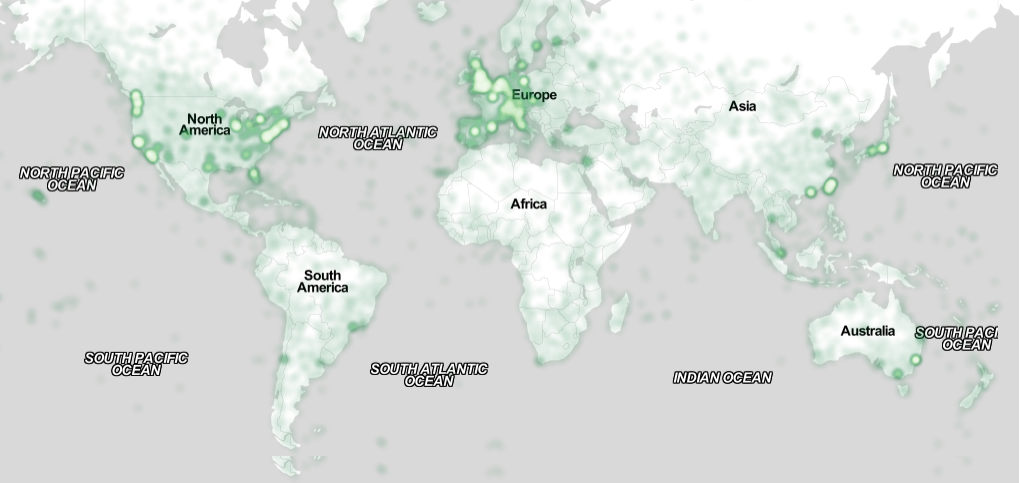
\includegraphics[width=0.9\columnwidth]{map.png}
  \caption{Insert a caption below each figure.}~\label{fig:sample}
  \end{centering}
\end{figure}

\subsection{Tables}
For an example, see Table~\ref{tab:table1}. Try to
minimize the use of lines (especially vertical lines). \LaTeX\ will
set the table font and captions sizes correctly.

\begin{table}
  \centering
  \begin{tabular}{l r r r}
    % \toprule
    & & \multicolumn{2}{c}{\small{\textbf{Test Conditions}}} \\
    \cmidrule(r){3-4}
    {\small\textit{Name}}
    & {\small \textit{First}}
      & {\small \textit{Second}}
    & {\small \textit{Final}} \\
    \midrule
    Marsden & 223.0 & 44 & 432,321 \\
    Nass & 22.2 & 16 & 234,333 \\
    Borriello & 22.9 & 11 & 93,123 \\
    Karat & 34.9 & 2200 & 103,322 \\
    % \bottomrule
  \end{tabular}
  \caption{Table captions should be placed below the table. We
    recommend table lines be 1 point, 25\% black. Minimize use of
    table grid lines.}~\label{tab:table1}
\end{table}

\section{Citing and Formatting References}

Any references should be published materials accessible to the
public. Private communications
should be acknowledged in the main text, not referenced (e.g.,
[Blau, personal communication]). References must be the same
font size as other body text. References should be in alphabetical
order by last name of first author, then by year and title. Use a numbered list of references
at the end of the article, ordered alphabetically by last name of
first author, and referenced by numbers in brackets. For papers from
conference proceedings, include the title of the paper and the name of
the conference, as well as page numbers and DOI if available.

References should be in ACM citation format:
\url{http://www.acm.org/publications/submissions/latex_style}.  This
includes citations to Internet
resources~\cite{cavender:writing,CHI,CHINOSAUR:venue,OED:they,psy:gangnam}
according to ACM format, although it is often appropriate to include
URLs directly in the text, as above. Example reference formatting for
individual journal articles~\cite{ethics}, articles in conference
proceedings~\cite{Klemmer:2002:WSC:503376.503378},
books~\cite{Schwartz:1995:GBF}, theses~\cite{sutherland:sketchpad},
book chapters~\cite{winner:politics}, an entire journal
issue~\cite{kaye:puc},
websites~\cite{acm_categories,cavender:writing},
tweets~\cite{CHINOSAUR:venue}, patents~\cite{heilig:sensorama}, 
games~\cite{supermetroid:snes}, and
online videos~\cite{psy:gangnam} is given here.  See the examples of
citations at the end of this document and in the accompanying
\texttt{BibTeX} document.

\section{Acknowledgements}
This template was initially prepared by Janet Davis.
I thank Amy Blau at Penrose Library for her guidance on appropriate formatting and  CS major Cooper Lazar for his help with researching PDF/A document production. I also thank all the SIGCHI volunteers, publications support, staff, and authors
who developed the CHI Proceedings Format~\cite{CHI}. 

Remember to thank your project supervisor, your team, your client, and any research participants, as well as others who helped or supported you.

\printbibliography

\end{document}
